\documentclass[11pt]{article}

\usepackage[margin=1in]{geometry}
\usepackage{amsmath, amssymb, amsthm}
\usepackage{mathtools}
\usepackage{enumitem}
\usepackage{booktabs}
\usepackage{array}
\usepackage{hyperref}
\usepackage{xcolor}
\usepackage{microtype}
\usepackage{algorithm}
\usepackage{algpseudocode}
\usepackage{graphicx}
\usepackage{float}


\hypersetup{
    colorlinks=true,
    linkcolor=blue!60!black,
    citecolor=blue!60!black,
    urlcolor=blue!60!black
}

\newtheorem{definition}{Definition}
\newtheorem{theorem}{Theorem}
\newtheorem{proposition}{Proposition}
\newtheorem{observation}{Observation}
\newtheorem{question}{Research Question}

\title{Empirical and Theoretical Study of Pivot-Augmented LSH Forest for Approximate Nearest Neighbor Search}
\author{Aditya Jhaveri (aaj6301) \and Bhavik Patwa (bnp7995)}
\date{May 2026}

\begin{document}
\maketitle

\begin{abstract}
Approximate nearest neighbor search is a central problem in high-dimensional algorithms, where exact methods often become infeasible due to the curse of dimensionality. Our foundational paper, \emph{LSH Forest : Practical Algorithms Made Theoretical} by Andoni, Razenshteyn and Nosatzki, studies a widely used nearest-neighbor heuristic and proves that a simple pivot-augmented variant of LSH Forest can outperform classical data-oblivious locality-sensitive hashing in Hamming space. The paper is theoretically important because it bridges a gap between practical heuristics and provable data-dependent hashing guarantees.

This project combines a digestible exposition of the paper's main theoretical ideas with a theory-informed empirical study of the pivot parameter $k$. We investigate how increasing the number of pivots per node affects recall, query latency, candidate comparisons, pivot comparisons, traversal depth, build cost and a memory proxy across several synthetic binary dataset regimes. We implemented three methods : bit-sampling LSH, vanilla LSH Forest and a simplified pivot-augmented LSH Forest prototype. Our experiments show that increasing $k$ changes the internal behavior of the forest in a way qualitatively consistent with the paper's structural intuition : it tends to reduce traversal depth and candidate comparisons while increasing pivot work, build time and memory use. However, these structural improvements do not uniformly translate into faster queries. Bit-sampling LSH remains strongest on random binary data, forest-based methods improve recall on clustered data but do not surpass bit-sampling LSH in query time and forest-based methods substantially outperform bit-sampling on sparse binary data. We also discuss a natural Euclidean generalization and explain why the Hamming proof does not transfer directly : the original analysis relies on coordinate-wise concentration, while Euclidean random projections and centroids do not provide the same combinatorial structure.
\end{abstract}

\section{Introduction}

Nearest neighbor search asks us to preprocess a dataset $P$ of $n$ points so that, given a query $q$, we can quickly return a point of $P$ close to $q$. In high dimensions, exact nearest neighbor search is often too expensive, so both theory and practice rely on approximate near neighbor search.

\begin{definition}[$(c,r)$-Approximate Near Neighbor]
Let $(X,D)$ be a metric space, let $P \subseteq X$ be a dataset and let $c>1$. A data structure solves the $(c,r)$-approximate near neighbor problem if, whenever there exists $p^* \in P$ with $D(p^*,q) \le r$, the data structure returns some $p \in P$ satisfying
\[
    D(p,q) \le cr.
\]
\end{definition}

Locality-sensitive hashing (LSH), introduced by Indyk and Motwani, is one of the most influential approaches to approximate nearest neighbor search. An LSH family hashes points so that near pairs collide with higher probability than far pairs. If the collision probability for near pairs is $p_1$ and the collision probability for far pairs is $p_2$, then the performance of the construction is governed by the exponent
\[
    \rho = \frac{\log(1/p_1)}{\log(1/p_2)}.
\]
Smaller values of $\rho$ correspond to better asymptotic query time. Classical data-oblivious LSH in Hamming space achieves an exponent essentially equal to $1/c$, while more complex data-dependent hashing methods can improve this bound.

The paper \emph{LSH Forest : Practical Algorithms Made Theoretical} asks whether a simple practical data structure, already used as a heuristic, can be modified just enough to obtain a provable data-dependent improvement. The answer is yes for Hamming space. The authors augment LSH Forest with carefully chosen pivots at tree nodes and show that this modification achieves
\[
    \rho \le \frac{1}{\ln 4}\cdot \frac{1}{c}\left(1+O\left(\frac{1}{k}\right)\right) + O\left(\frac{1}{c^2}\right),
\]
where $k$ is the number of pivots stored per node. Since $1/\ln 4 \approx 0.721$, this improves over the classical Hamming-space exponent $1/c$ while remaining much simpler than the best known optimal data-dependent hashing methods.

This study has two goals. First, we explain the main theoretical intuition behind pivot-augmented LSH Forest in a digestible way. Second, we empirically investigate a natural question left open by the theory : how should the pivot count $k$ be chosen in practice? The theorem improves as $k$ grows, but larger $k$ also increases pivot comparisons, build time and space usage. Thus, the empirical question is not simply whether one algorithm is faster than another. Rather, it is whether a theoretically meaningful structural parameter creates useful practical tradeoffs under different dataset regimes.

\section{Background : LSH and LSH Forest}

\subsection{Classical bit-sampling LSH in Hamming space}

For Hamming space $\{0,1\}^d$, the simplest LSH family is bit sampling. A hash function chooses a coordinate $i \in [d]$ uniformly at random and maps
\[
    h_i(x) = x_i.
\]
For two points $x,y \in \{0,1\}^d$ with Hamming distance $\|x-y\|_1$, the collision probability is
\[
    \Pr[h_i(x)=h_i(y)] = 1 - \frac{\|x-y\|_1}{d}.
\]
Thus, if near points have distance at most $r$ and far points have distance at least $cr$, then
\[
    p_1 = 1 - \frac{r}{d}, \qquad p_2 = 1 - \frac{cr}{d}.
\]
The LSH exponent is
\[
    \rho = \frac{\log(1/p_1)}{\log(1/p_2)}.
\]
In the worst case, this behaves like $1/c$ and this bound is tight for data-oblivious Hamming LSH. The classical construction concatenates several independent hashes to reduce far collisions and repeats the table many times to preserve near collisions. The resulting query time is roughly $n^\rho$ up to dimension and logarithmic factors, while space is roughly $n^{1+\rho}$.

\subsection{Vanilla LSH Forest}

LSH Forest can be viewed as replacing fixed-length hash tables with trie-like structures. For Hamming space, choose a random permutation $\pi$ of the coordinates and insert every point $x \in P$ as the permuted string
\[
    x_{\pi(1)}, x_{\pi(2)}, \ldots, x_{\pi(d)}.
\]
The trie branches according to coordinate values. A query follows the same coordinate order down the trie until it reaches a leaf or a missing branch. Unlike fixed-length LSH, different parts of the dataset can be separated at different depths. This adaptivity is the source of LSH Forest's practical appeal.

However, vanilla LSH Forest does not improve the worst-case exponent. There are inputs where its random coordinate splits behave no better than bit-sampling LSH, so one still needs about $n^{1/c}$ independent trees. The key contribution of the foundational paper is to show that a small data-dependent augmentation can change this worst-case behavior.

\section{Pivot-Augmented LSH Forest}

The central idea of Andoni, Razenshteyn and Nosatzki is simple : at every node of the trie, store a small number of representative pivots from the subset of points reaching that node. During a query, when the algorithm visits a node, it checks the query against the stored pivots before continuing downward.

\begin{algorithm}[h]
\caption{Pivot-Augmented Query in One Tree}
\begin{algorithmic}[1]
\Require Tree node $v$, query $q$, approximation factor $c$, radius $r$
\For{each pivot $p \in T_v$ stored at node $v$}
    \If{$D(p,q) \le cr$}
        \State \Return $p$
    \EndIf
\EndFor
\If{there exists a child $u$ of $v$ matching the next hash or partition value of $q$}
    \State \Return Query$(u,q)$
\Else
    \State \Return $\bot$
\EndIf
\end{algorithmic}
\end{algorithm}

The pivots are chosen so that they are close to the center of the local subset. In Hamming space, the natural notion of center is the coordinate-wise mean. If $S \subseteq \{0,1\}^d$ is the set of points at a node, define
\[
    \mu(S)_j = \frac{1}{|S|}\sum_{x \in S} x_j.
\]
The algorithm greedily selects $k$ points in $S$ that are close to this mean while remaining sufficiently diverse. Intuitively, these pivots represent the dense central portion of the current node.

\subsection{Why pivots help}

Random coordinate splitting is bad when the near neighbor and query differ on an early selected coordinate. Vanilla LSH Forest simply loses the near neighbor in that tree. Pivot-augmented LSH Forest has a second chance : even if the query is about to be separated from its true near neighbor, a stored pivot may already be within distance $cr$ and therefore be a valid approximate answer.

The proof analyzes the expected progress of the query through the tree. Roughly, the algorithm succeeds when either :
\begin{enumerate}[leftmargin=*]
    \item the query and the true near neighbor remain together long enough, or
    \item before they separate, one of the stored pivots is already a valid $cr$-approximate answer.
\end{enumerate}
This second success mode is not available in standard LSH. It is the source of the data-dependent gain.

\subsection{Main theorem}

The paper's main theorem can be stated informally as follows.

\begin{theorem}[Andoni, Razenshteyn and Nosatzki]
For Hamming space $\{0,1\}^d$, pivot-augmented LSH Forest with $k$ pivots per node solves $(c,r)$-ANN using $O(n^\rho)$ independent trees, where
\[
    \rho \le \frac{1}{\ln 4}\cdot \frac{1}{c}\left(1+O\left(\frac{1}{k}\right)\right)+O\left(\frac{1}{c^2}\right).
\]
For sufficiently large $k$, this is approximately $0.721/c$, improving over the classical Hamming LSH exponent $1/c$.
\end{theorem}

The theorem captures the central tradeoff of the method. As $k$ increases, the exponent improves toward its limiting value. However, larger $k$ also increases the number of pivots checked at query time and the amount of information stored in the data structure. The query time is of the form
\[
    O(n^\rho d^2 k),
\]
and the space is roughly
\[
    O(n^{1+\rho}k + nd),
\]
up to implementation conventions and lower-order factors.

\section{Simplified Proof Intuition}

The proof is technical, but the main idea can be understood through a structured versus unstructured dichotomy.

\subsection{The random-data benchmark}

For bit-sampling LSH, the worst case occurs when $r/d$ is small. But if the distance scale is around
\[
    r \approx \frac{d}{2c},
\]
then the exponent becomes
\[
    \rho \approx \frac{\log 2}{\log(1/(1-1/(2c)))} \approx \frac{1}{\ln 4}\cdot \frac{1}{c}.
\]
This is the same constant improvement achieved by the pivot-augmented forest. One way to interpret the result is that pivot-augmented LSH Forest reduces difficult Hamming inputs to a more random-like regime for bit sampling.

\subsection{The role of the local mean}

For a node subset $S$, coordinates can be classified according to how biased they are. If many coordinates are heavily biased, then the points in $S$ are concentrated around their mean and a few well-chosen pivots can cover the useful central region. If coordinates are not heavily biased, then random coordinate splitting behaves more like the random-data case, where bit sampling already has the improved $1/(\ln 4)c$ behavior.

This creates the following dichotomy :
\begin{enumerate}[leftmargin=*]
    \item \textbf{Structured node :} points are concentrated near the mean, so pivots are useful.
    \item \textbf{Unstructured node :} random splitting is already good enough.
\end{enumerate}
Vanilla LSH Forest cannot use this dichotomy because it does not store central representatives. It only follows coordinate splits. Pivot augmentation converts local structure into actual candidate answers.

\section{Research Questions}

The primary empirical question we investigate is :

\begin{question}
How does the pivot count $k$ affect the practical behavior of pivot-augmented LSH Forest in Hamming space and to what extent are empirical trends qualitatively consistent with the paper's structural tradeoff between improvement and added cost?
\end{question}

This question is more substantial than asking whether one algorithm is faster than another. The parameter $k$ is central to the theorem : increasing $k$ improves the asymptotic bound, but also incurs greater query and space overhead. The empirical challenge is to determine whether this asymptotic story leads to meaningful practical improvements and, if so, under which dataset regimes.

We break this broad question into five subquestions :
\begin{enumerate}[leftmargin=*]
    \item Does increasing $k$ improve recall or search success behavior in practice?
    \item Does increasing $k$ reduce traversal depth or candidate comparisons, as the structural intuition suggests?
    \item At what point does increasing $k$ stop helping because pivot comparisons, build time and memory overhead dominate?
    \item Are there dataset regimes where forest-based methods are practically preferable to bit-sampling LSH?
    \item Is the best value of $k$ stable across dataset families, or does it depend strongly on structure?
\end{enumerate}

\subsection{Future theoretical direction : Euclidean pivot forests}

A natural further question is whether pivot augmentation can be generalized to Euclidean space. The most natural analogue replaces Hamming-coordinate splits with random projection splits and replaces coordinate-wise means with Euclidean centroids. At a node $v$ with point subset $S_v \subseteq \mathbb{R}^d$, one could compute
\[
    \mu_v = \frac{1}{|S_v|}\sum_{x \in S_v}x,
\]
store the $k$ points closest to $\mu_v$ as pivots and split the node using a Gaussian random projection $g \sim N(0,I_d)$ with a median threshold :
\[
    x \mapsto \mathbf{1}\{\langle g,x\rangle \ge \tau_v\}.
\]

This algorithm is conceptually natural, but a direct proof appears difficult. The Hamming proof works because coordinate sampling, coordinate-wise means and coordinate bias all align. In Euclidean space, random projections mix all coordinates and centroid-near pivots may not cover queries lying along thin or anisotropic directions. A more plausible Euclidean variant would combine centroid pivots with covariance-aware directional pivots, for example by storing points with extreme projections along top principal directions. This suggests a future question : can pivot forests obtain guarantees on restricted Euclidean families such as low-rank clusters, bounded-doubling metrics, or structured embedding datasets? We do not solve this question, but identifying this barrier clarifies why the Hamming result is not simply a generic ``add pivots to any tree'' theorem.

\section{Approach and Methodology}

This study takes a theory-informed empirical approach. We do not attempt a new theorem or lower bound. Instead, we build a controlled prototype to study the parameter $k$ in a way that captures the main conceptual structure of the paper.

We implemented three methods :
\begin{enumerate}[leftmargin=*]
    \item bit-sampling LSH,
    \item vanilla LSH Forest,
    \item pivot-augmented LSH Forest prototype.
\end{enumerate}

The implementation was inspired by the structural interpretation of pivot augmentation described above. Our prototype is not a full reproduction of every technical detail in the original paper. The goal is clarity, instrumentation and control over the parameter $k$, rather than low-level optimization or exact reproduction of every asymptotic convention. This distinction is important : the purpose of the prototype is to support careful comparative study, not to claim an industrial-strength implementation.

The full project code is available on GitHub at
\begin{center}
    \url{https://github.com/swooshie/pivot-augmented-lsh-forest-study.git}.
\end{center}
The repository contains the Python implementations of bit-sampling LSH, vanilla LSH Forest and the pivot-augmented LSH Forest prototype, along with synthetic Hamming-space dataset generators, experiment scripts, analysis scripts and instructions for reproducing the reported measurements and figures.

The experimental evaluation measures :
\begin{itemize}[leftmargin=*]
    \item recall,
    \item average query time in milliseconds,
    \item average nodes visited,
    \item average pivot comparisons,
    \item average candidate comparisons,
    \item average traversal depth,
    \item build time,
    \item a memory proxy based on stored structure size.
\end{itemize}

The memory quantity is a structural proxy for index size, not a direct measurement of true RAM consumption. We use it to compare relative growth across methods and pivot counts. Experiments were repeated over multiple random seeds to reduce the chance that conclusions reflect a single lucky or unlucky trial.

\section{Implementation Details}

The code was written in Python and organized as a small research codebase. The bit-sampling LSH baseline uses random coordinate subsets as hash signatures. At query time, it probes matching buckets across several hash tables and checks candidate points using Hamming distance.

The vanilla LSH Forest implementation uses random permutations of coordinates and recursively splits points according to those coordinate orders, producing trie-like structures. Queries descend along a path induced by the query's bit values. Candidate checking occurs at leaves.

The pivot-augmented LSH Forest extends this structure by adding up to $k$ pivots at each node. The pivots are selected using a simplified version of the paper's idea : points are prioritized by nearness to the mean of the node's subset, while also satisfying a separation condition so that pivots are sufficiently diverse. During query processing, the query is compared against pivots stored at every visited node. If a pivot lies within the approximation threshold, the query succeeds immediately.

Initial experimental settings were not sufficiently discriminating, so the final study used stronger dataset regimes and more detailed instrumentation. In particular, we refined the prototype in several ways :
\begin{itemize}[leftmargin=*]
    \item strengthened the dataset design,
    \item added repeated seeds and aggregated summaries,
    \item improved candidate accounting,
    \item reported build cost and a memory proxy,
    \item made the forest construction closer to the paper's random-permutation trie idea.
\end{itemize}
These refinements made the final study more credible and better aligned with the theoretical motivation.

\section{Experimental Design}

A major design choice was to use multiple synthetic dataset families rather than only one. This matters because the foundational paper is about Hamming-space structure and different binary regimes can induce very different search behavior.

We used three synthetic dataset families.

\paragraph{Random binary data.} Each point is generated independently and uniformly in $\{0,1\}^d$ and queries are created by flipping a fixed number of bits of sampled dataset points. This serves as a natural control regime and is relatively favorable to simple hashing methods.

\paragraph{Clustered binary data.} A set of binary cluster centers is generated and each data point is formed by perturbing one cluster center. Queries are then formed by perturbing dataset points. This regime introduces local geometric structure, which should be more favorable to adaptive tree-based methods.

\paragraph{Sparse binary data.} Each point has only a small number of active bits. Queries again arise by small perturbations. This regime is revealing because bucket-based methods can become burdened by larger effective candidate sets even when recall remains high.

Our larger experiment used datasets with $4000$ points, $300$ queries and $256$ dimensions. The approximation factor was set to $2.0$. The pivot counts examined were
\[
    k \in \{1,2,4,8\}.
\]
The number of trees was set to $12$ and experiments were repeated across three random seeds. This setup does not exhaust all possible regimes, but it is adequate to support a meaningful study of tradeoffs.

\section{Results}

Our final experiments produced a stable and interpretable picture. Figure~\ref{fig:method-tradeoffs} summarizes the main cross-method comparison for each dataset family, while Figure~\ref{fig:pivot-scaling} shows how query time, build time, and memory proxy scale with the pivot count $k$ within the forest family. The main results are summarized in Table~\ref{tab:summary}.

\begin{table}[h]
\centering
\caption{Summary of observed performance trends across dataset regimes. Query times are mean values from the final experiments.}
\label{tab:summary}
\begin{tabular}{@{}p{0.17\textwidth}p{0.22\textwidth}p{0.18\textwidth}p{0.33\textwidth}@{}}
\toprule
Dataset regime & Strongest method by time & Recall pattern & Main observation \\
\midrule
Random binary & Bit-sampling LSH & All methods $1.0$ & Pivots add overhead after recall saturates \\
Clustered binary & Bit-sampling LSH & Forest methods $1.0$ & Forests improve recall but not time \\
Sparse binary & Vanilla or small-$k$ forest & All methods $1.0$ & Forest traversal beats bucket-heavy LSH \\
\bottomrule
\end{tabular}
\end{table}

\begin{figure}[H]
    \centering
    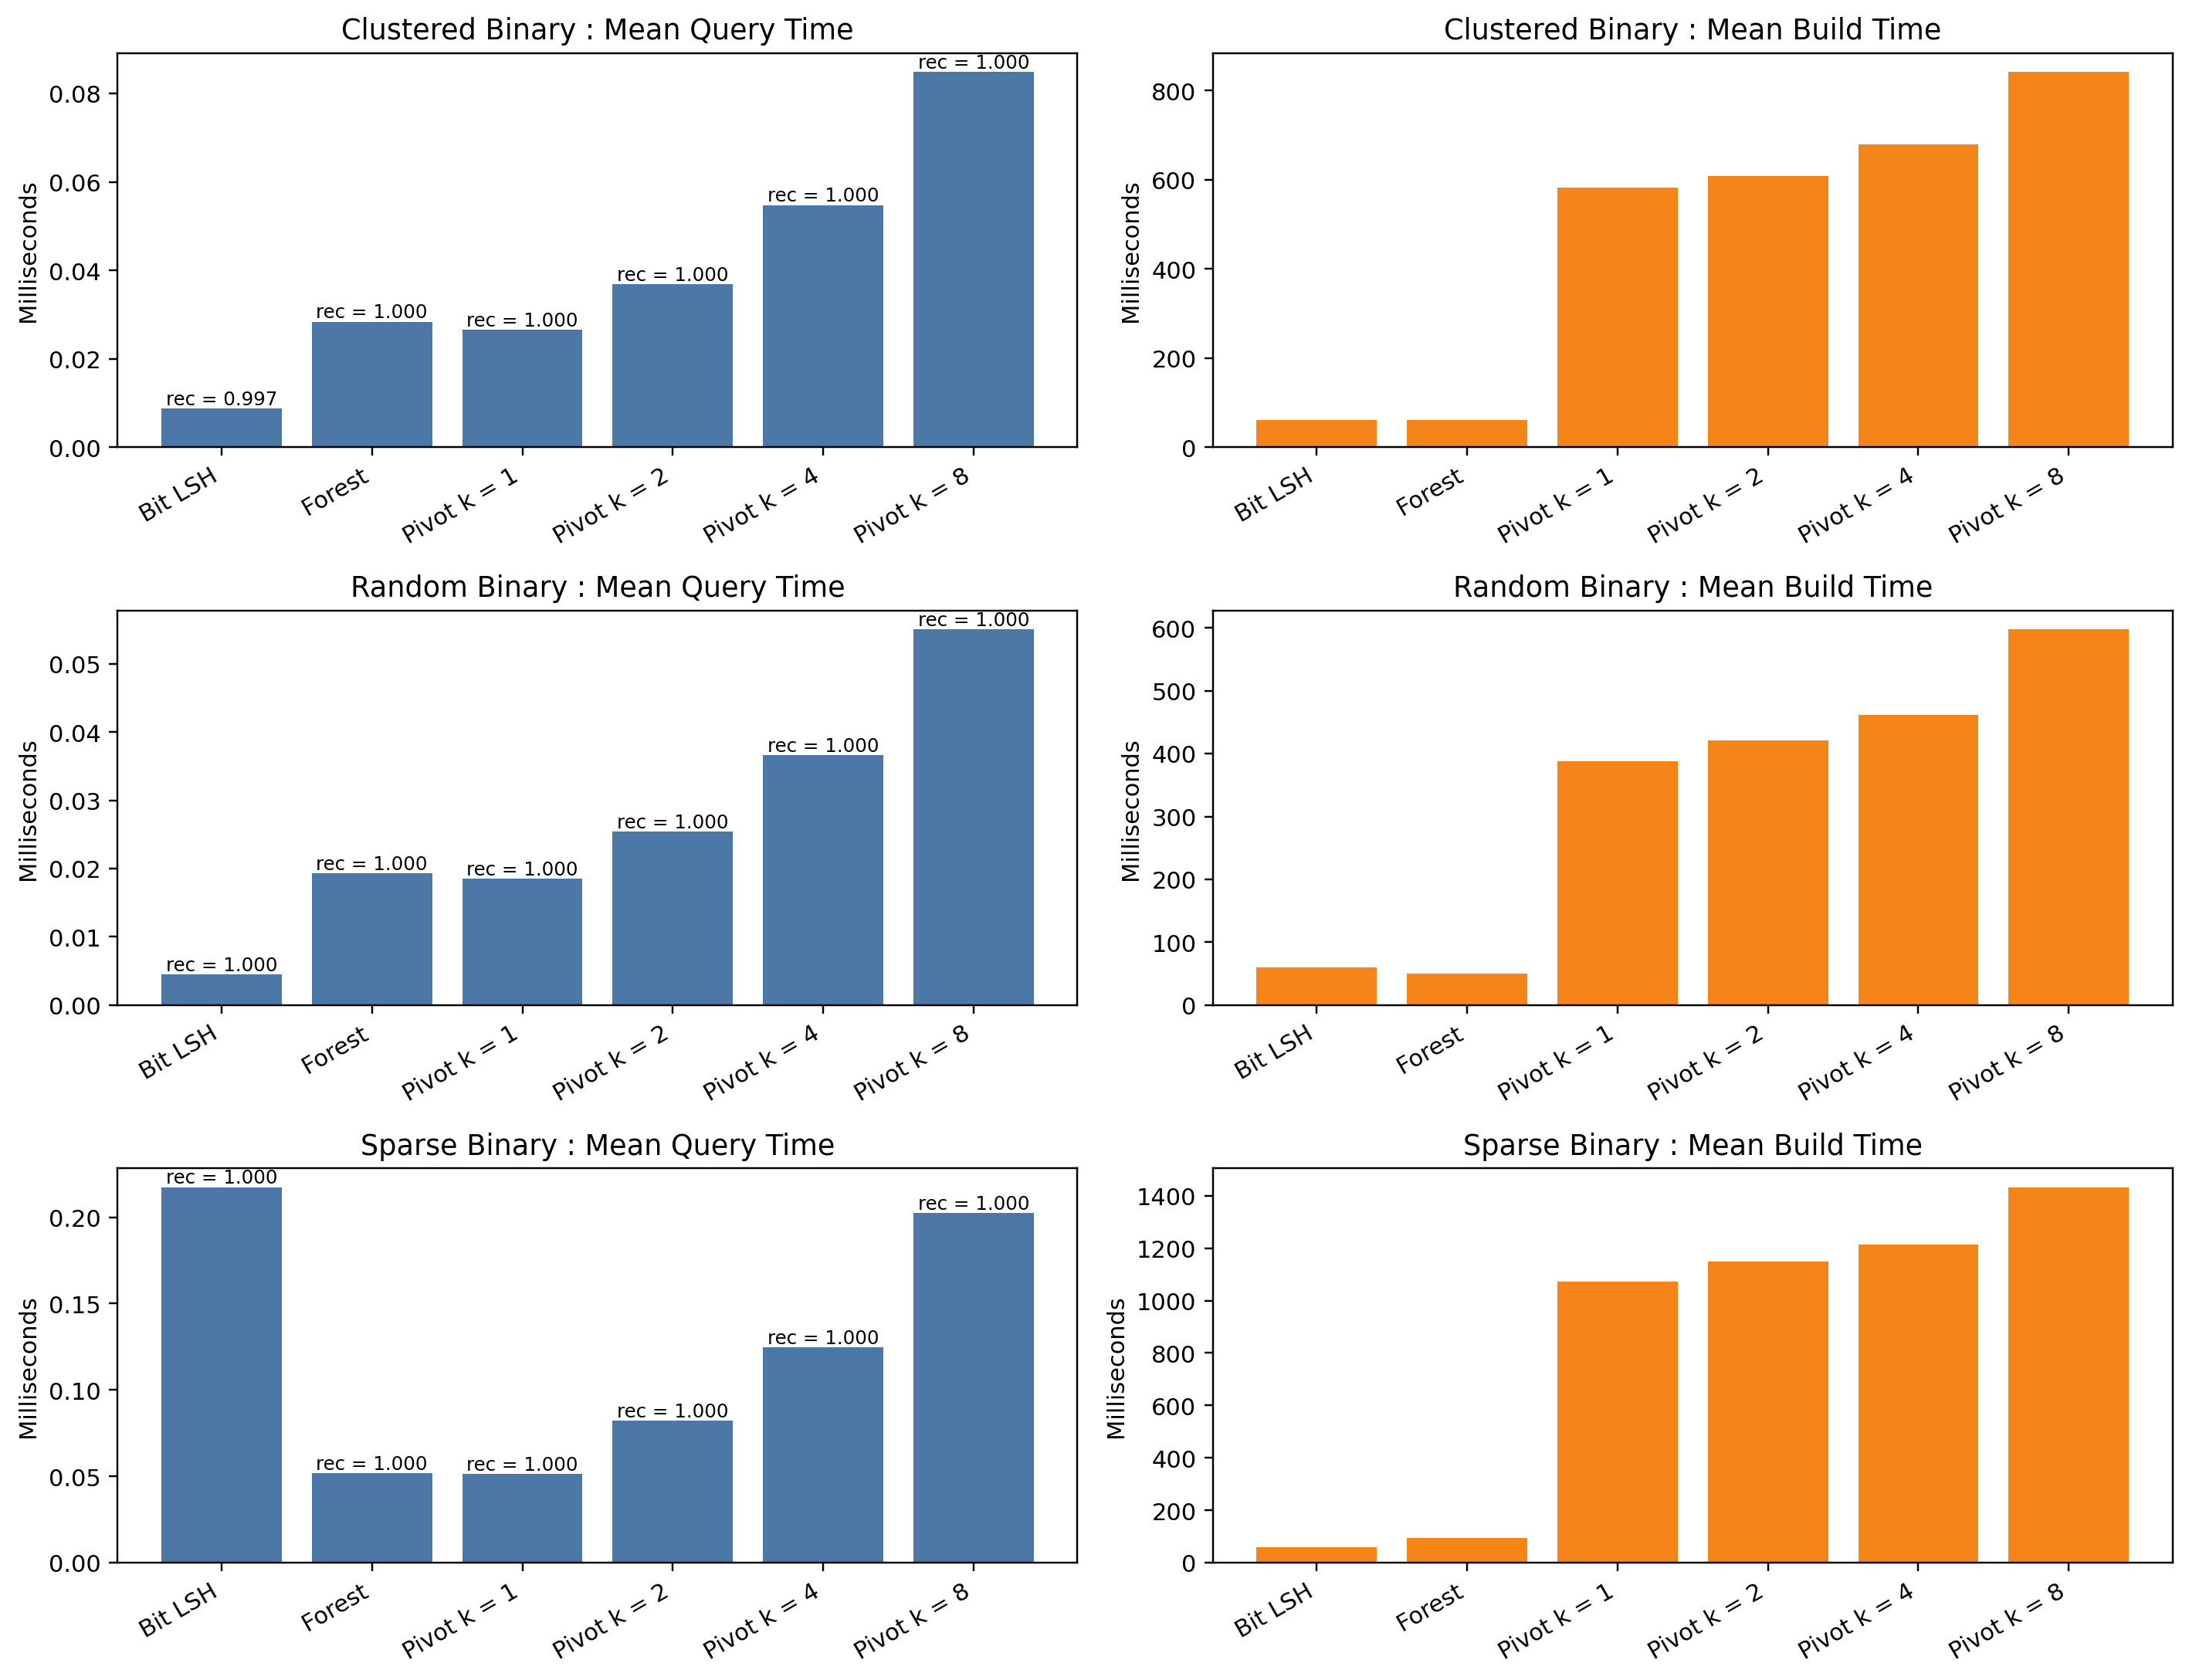
\includegraphics[width=\textwidth]{figure_method_tradeoffs.png}
    \caption{Per-dataset comparison of mean query time and mean build time across Bit LSH, vanilla LSH Forest and pivot-augmented LSH Forest prototype with different pivot counts. Recall annotations are shown above the query-time bars. The figure highlights that the practical ranking of methods depends strongly on dataset regime : Bit LSH is fastest on random binary data, while forest-based methods are substantially faster on sparse binary data.}
    \label{fig:method-tradeoffs}
\end{figure}

\subsection{Random binary data}

On random binary data, all methods achieved perfect recall. Bit-sampling LSH had the best query time by a large margin, with mean query time around $0.0047$ ms. Vanilla LSH Forest was slower, at about $0.0198$ ms and pivot-augmented variants became progressively slower as $k$ increased. For example, $k=8$ yielded mean query time around $0.0552$ ms.

Increasing $k$ reduced traversal depth and candidate comparisons, but because recall was already saturated and the baseline was extremely strong, these structural improvements did not lead to a practical win. This is an important negative result. It shows that in a regime resembling random binary instances, the simplicity and efficiency of bit-sampling LSH are hard to beat.

This pattern is clearly visible in Figure~\ref{fig:method-tradeoffs}, where Bit LSH dominates in query time while larger pivot counts incur steadily increasing cost.

\subsection{Clustered binary data}

On clustered binary data, the picture was somewhat different. Bit-sampling LSH had mean recall approximately $0.9967$, while vanilla LSH Forest and all pivot-augmented variants achieved recall $1.0$ in all repeated runs. However, the forest-based methods were still slower in wall-clock terms. Vanilla LSH Forest had mean query time about $0.0274$ ms, while pivot variants ranged from about $0.0267$ ms for $k=1$ to $0.0834$ ms for $k=8$.

As before, increasing $k$ reduced nodes visited and candidate comparisons, but the added pivot work dominated query time. The clustered regime therefore supports an intermediate conclusion : the forest family appears structurally well-suited to the data, but the practical benefit of larger $k$ is limited once recall has already saturated.

\subsection{Sparse binary data}

The sparse binary regime is the most interesting. In this case, all methods again achieved perfect recall, but query-time behavior differed sharply. Bit-sampling LSH was much slower than in the other regimes, with mean query time about $0.2115$ ms. By contrast, vanilla LSH Forest achieved about $0.0519$ ms and pivot $k=1$ performed similarly. Larger $k$ values gradually increased latency, but the forest family still clearly outperformed bit-sampling LSH for modest $k$.

This sparse-binary result is the strongest empirical finding in the project. It shows that the practical story is not simply that bit-sampling LSH wins overall. Instead, the right algorithm depends strongly on dataset regime. Forest methods can be practically advantageous in some settings and larger $k$ is not automatically the right choice once recall is already perfect.

Figure~\ref{fig:method-tradeoffs} makes this contrast especially clear: sparse binary data is the regime in which the forest-based methods become substantially faster than Bit LSH in query latency.

\begin{figure}[H]
    \centering
    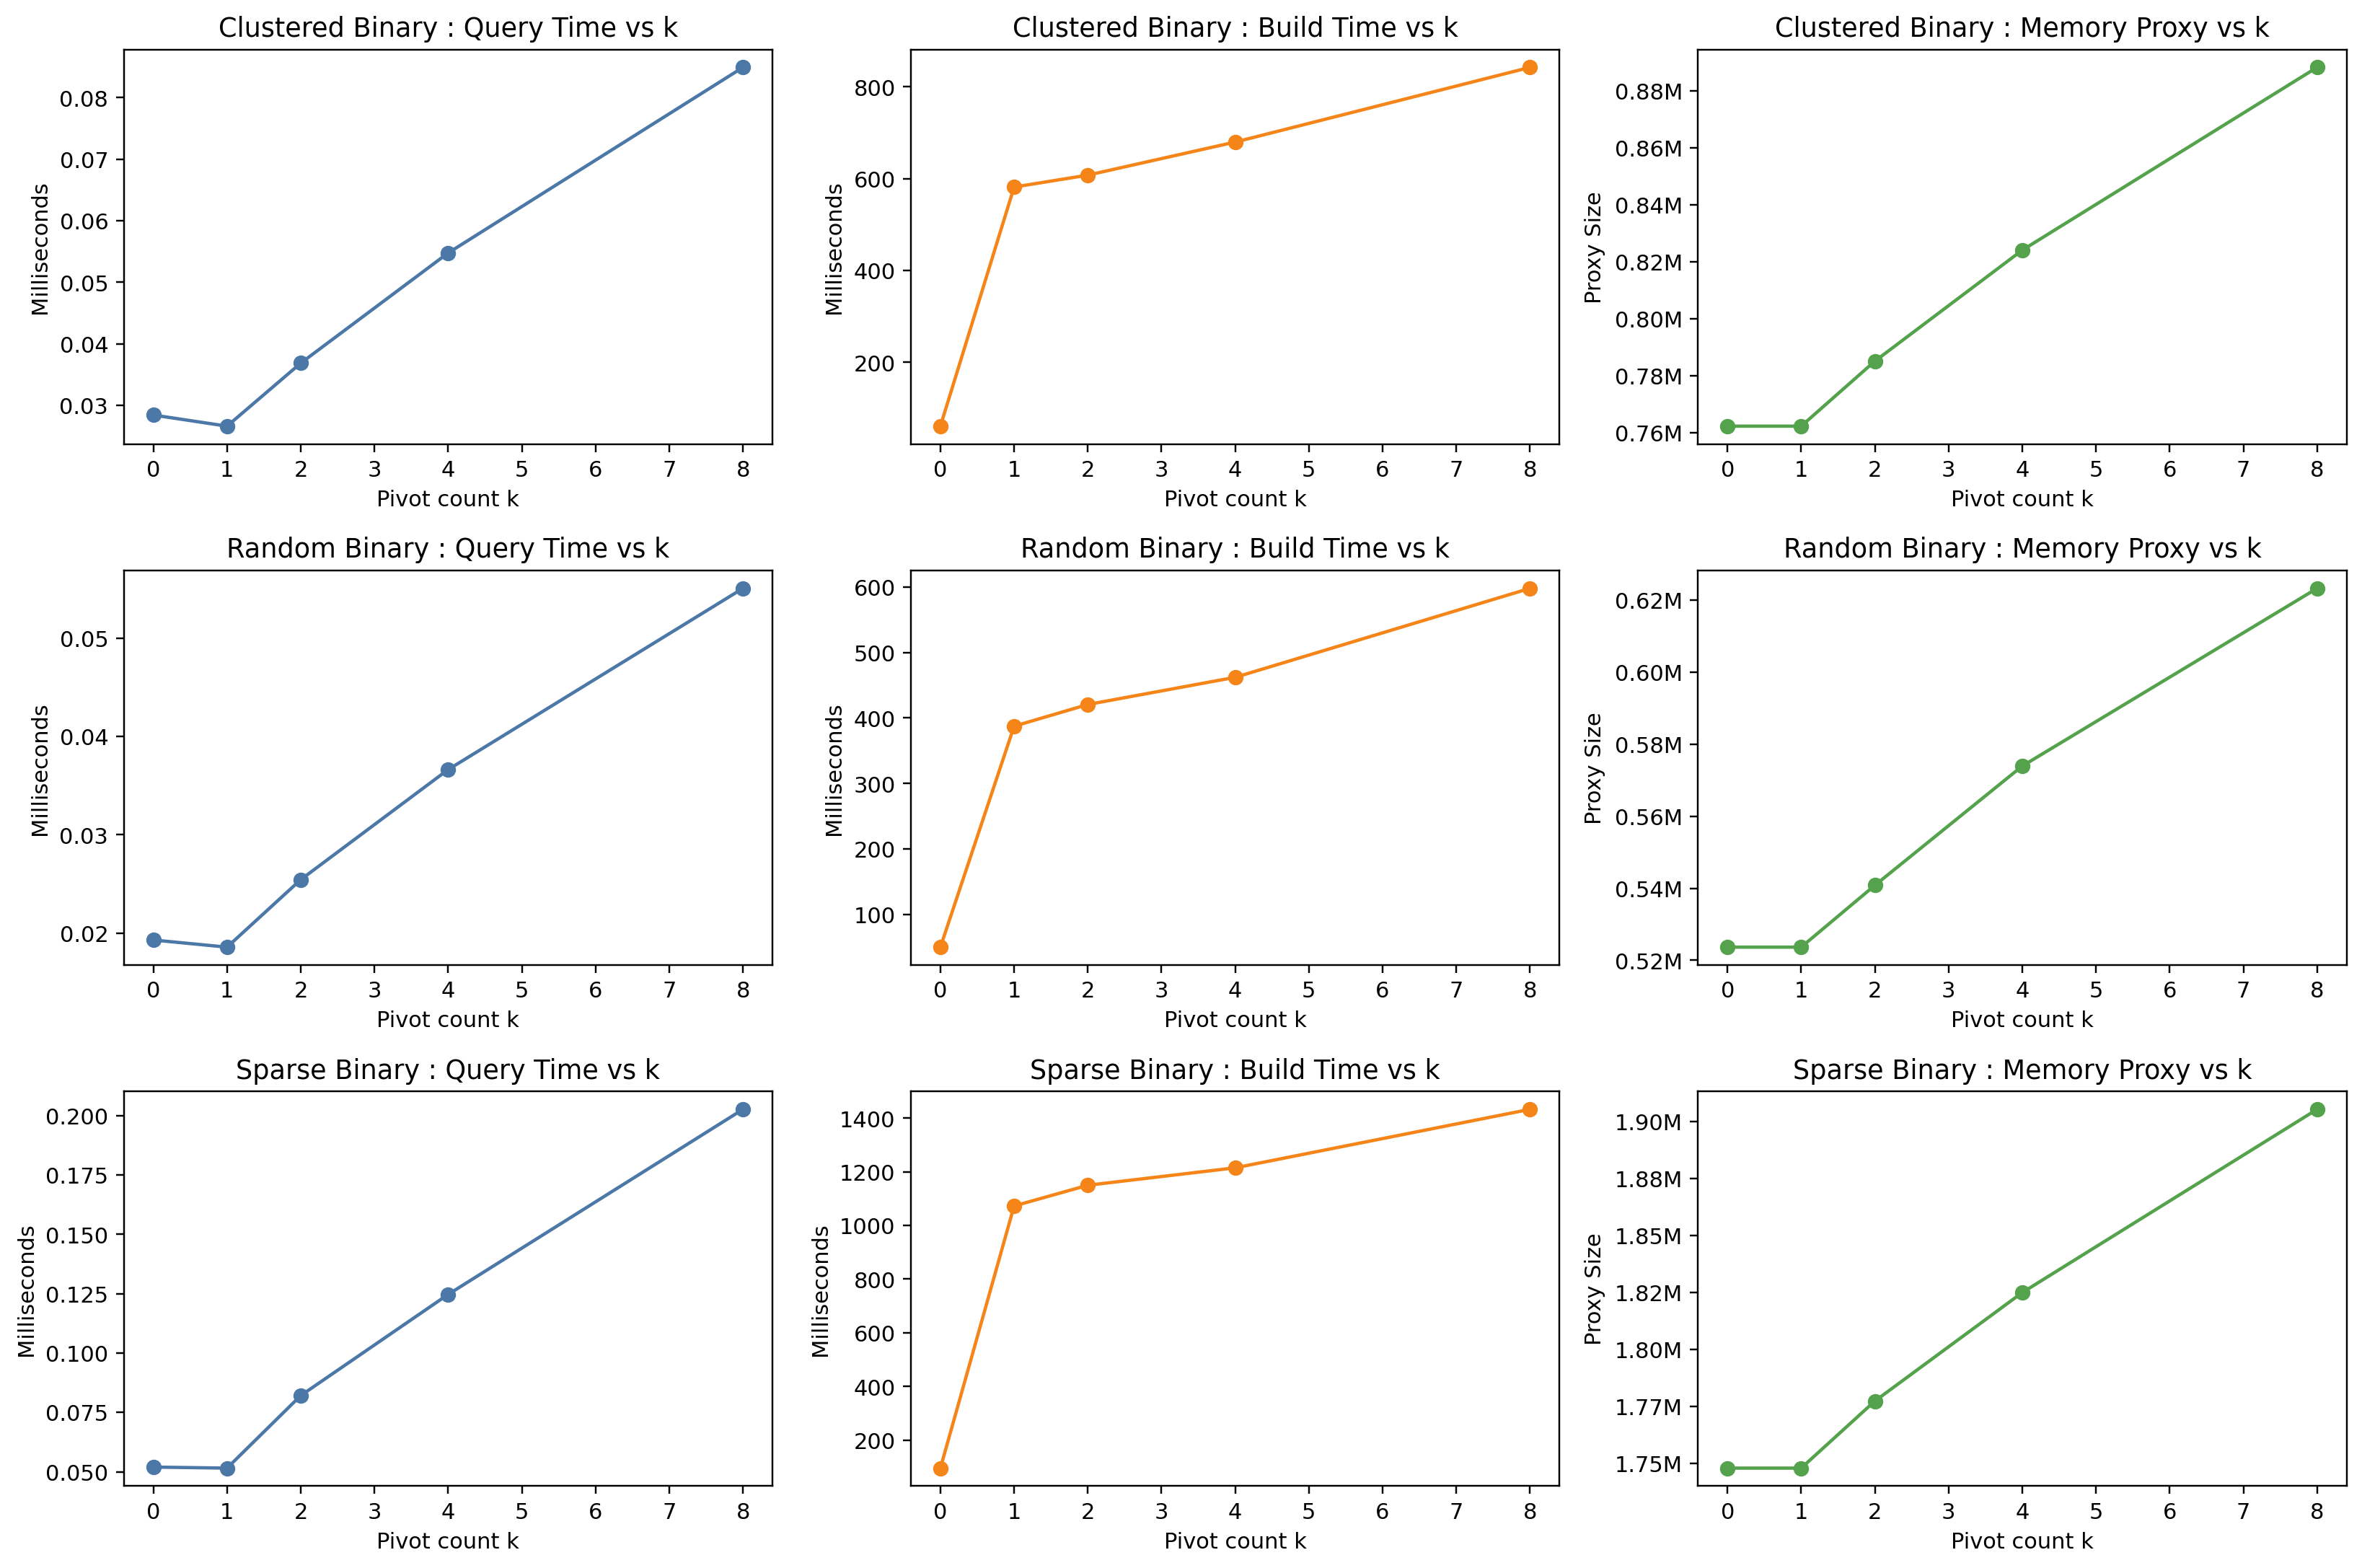
\includegraphics[width=\textwidth]{figure_pivot_scaling.png}
    \caption{Scaling behavior of the forest family as the pivot count $k$ increases. For each dataset family, the figure reports mean query time, mean build time, and memory proxy. Increasing $k$ generally increases build cost and memory usage, while the effect on query time depends on dataset regime.}
    \label{fig:pivot-scaling}
\end{figure}

\subsection{Cross-regime trends}

Across all regimes, larger $k$ tends to reduce depth and candidate comparisons but increases pivot comparisons, build cost and the memory proxy. This is qualitatively the sort of tradeoff the theoretical paper suggests at a structural level. The safest interpretation is that our empirical findings are qualitatively consistent with the paper's structural intuition, even though our implementation is only a simplified research prototype.

Figure~\ref{fig:pivot-scaling} further shows that increasing $k$ produces a consistent growth in build time and memory proxy across all dataset families, even when the query-time benefits are limited or absent.

\section{Discussion}

The central question of this project was whether the pivot count $k$ has a meaningful empirical role and whether the paper's structural intuition about larger $k$ yields practical gains. The answer is nuanced.

First, the pivot mechanism clearly matters. Across experiments, increasing $k$ consistently changes the search process. It tends to reduce traversal depth, reduce candidate comparisons and make search more locally decisive. This is evidence that the structural intuition of the paper is qualitatively reflected in practice.

Second, the practical value of larger $k$ is limited by overhead. As $k$ grows, the algorithm performs many more pivot comparisons, uses more memory and requires more build time. In the current prototype, these costs rise quickly. Therefore, even when larger $k$ improves the internal search structure, it may not improve practical query time.

Third, practical performance is highly dataset-dependent. On random binary data, bit-sampling LSH remains extremely strong. On clustered binary data, the forest family becomes more competitive but still not clearly superior in time. On sparse binary data, forest-based methods become substantially better. This suggests that any practical recommendation about pivot-augmented LSH Forest should be conditioned on the geometric or combinatorial structure of the data, rather than stated universally.

Fourth, larger $k$ is not always better. This directly addresses the motivating question of this study. Theoretical asymptotics suggest that increasing $k$ improves the exponent, but empirical efficiency is more delicate. Once recall is already perfect, the marginal benefit of larger $k$ may be negligible, while the cost continues to grow. In the sparse regime, for example, $k=1$ is already competitive and larger $k$ mostly degrades runtime.

Overall, the experiments show that the research question was well chosen. The answer is not a simple win-or-lose outcome, but a structured tradeoff, which is exactly the kind of result an empirical algorithms project should aim for.

\section{Limitations and Barriers}

This project has several important limitations.

First, the code is a research prototype rather than a complete reproduction of the original paper. Although the later version is more faithful to the paper's forest structure than the earliest prototype, it still simplifies some implementation details. This is acceptable for the project's purpose, but it limits how strongly we can claim direct correspondence to the exact algorithm.

Second, the datasets are synthetic. This is not a fatal flaw, since synthetic data was useful for isolating structural effects, but it means that conclusions should be phrased as evidence about controlled binary regimes rather than evidence about all practical nearest-neighbor workloads.

Third, recall saturates quickly in many regimes. This makes runtime and structural metrics more important, but it also means that some comparisons are less discriminating than one might hope. A more extended project could explore harder query settings or lower tree budgets to obtain richer recall curves.

Fourth, the build time of pivot-augmented forests is large in the current implementation. This is itself a legitimate empirical finding, but it also reflects the fact that the prototype prioritizes interpretability over optimization.

Fifth, the study does not attempt theoretical proofs beyond the foundational paper. This study contributes empirical understanding and explanatory synthesis rather than a new theorem.

A practical barrier was that simpler experimental settings did not yield sufficiently informative comparisons. The earliest experiment design used easier data regimes and more limited instrumentation. We therefore revised both the implementation and methodology before treating the final results as credible. This revision process strengthened the project and is part of an honest research account of what we tried and what we learned.

\section{Future Work}

The most immediate empirical extension would be to evaluate the same algorithms on real-world binary or binarized embedding datasets, such as image descriptors or text embeddings after thresholding. This would help determine whether the sparse and clustered regimes observed in synthetic data appear in realistic workloads.

A second direction is to optimize the implementation. The prototype was designed for instrumentation, not speed. A more optimized implementation could use bit-packed Hamming distance computations, vectorized pivot checks and better memory layout. This would help separate algorithmic overhead from Python-level overhead.

A third direction is to study adaptive choices of $k$. Since larger $k$ helps some nodes more than others, a practical system might choose $k$ based on node size, coordinate bias, or local sparsity. This would be closer to the spirit of LSH Forest as a self-tuning data structure.

A fourth direction is the Euclidean extension discussed earlier. A centroid-only pivot strategy is probably too weak in anisotropic datasets, but covariance-aware directional pivots may be promising for structured Euclidean data. A useful theoretical target would be a guarantee for mixtures of low-rank clusters or bounded-doubling subsets, rather than all Euclidean datasets.

\section{Conclusion}

This project began with a deep reading of \emph{LSH Forest : Practical Algorithms Made Theoretical} and developed a new empirical question around one of its key parameters : the number of pivots per node, $k$. Our goal was not simply to test whether one algorithm is faster than another, but to understand how a theoretically meaningful structural parameter influences practical behavior.

The theoretical part of the project explains why pivot augmentation improves over vanilla LSH Forest in Hamming space. The key idea is a structured versus unstructured dichotomy : if a node is structured, pivots can directly provide valid approximate answers; if it is unstructured, random coordinate splitting is already close to the favorable random-data regime. This gives a clean intuition for the improved exponent of approximately $0.721/c$.

The empirical part shows that pivot augmentation has real consequences. Increasing $k$ changes the internal search structure in ways qualitatively consistent with the motivating theory, reducing traversal depth and candidate comparisons while increasing pivot work, build cost and memory overhead. However, these structural improvements do not uniformly translate into faster queries. On random binary data, bit-sampling LSH remains strongest. On clustered binary data, forest-based methods achieved perfect recall while bit-sampling LSH was slightly below perfect recall on average, but the forest-based methods remained slower. On sparse binary data, forest-based methods substantially outperformed bit-sampling in query latency.

The main conclusion is therefore not that pivot-augmented LSH Forest universally dominates classical baselines. Instead, this study supports a more mature claim : the practical value of pivot augmentation depends on dataset regime and larger $k$ is only worthwhile when its structural benefits outweigh its overhead. This directly addresses the unresolved practical question left open by the foundational paper.

Finally, the attempted Euclidean generalization clarifies why the result is specifically Hamming-theoretic rather than a generic pivot-tree theorem. The Hamming proof relies on coordinate-wise structure that does not transfer directly to Euclidean random projections. This gives a meaningful future direction and helps place the empirical results in a broader theoretical context.

\begin{thebibliography}{9}

\bibitem{arn2017}
Alexandr Andoni, Ilya Razenshteyn and Negev Shekel Nosatzki.
\newblock LSH Forest : Practical Algorithms Made Theoretical.
\newblock In \emph{Proceedings of the Twenty-Eighth Annual ACM-SIAM Symposium on Discrete Algorithms (SODA)}, pages 67--78, 2017.

\bibitem{indyk1998}
Piotr Indyk and Rajeev Motwani.
\newblock Approximate nearest neighbors : Towards removing the curse of dimensionality.
\newblock In \emph{Proceedings of the 30th ACM Symposium on Theory of Computing (STOC)}, pages 604--613, 1998.

\bibitem{andoni2015}
Alexandr Andoni and Ilya Razenshteyn.
\newblock Optimal data-dependent hashing for approximate near neighbors.
\newblock In \emph{Proceedings of the 47th ACM Symposium on Theory of Computing (STOC)}, pages 793--801, 2015.

\bibitem{andoni2016}
Alexandr Andoni and Ilya Razenshteyn.
\newblock Tight lower bounds for data-dependent locality-sensitive hashing.
\newblock In \emph{Proceedings of the 32nd International Symposium on Computational Geometry (SoCG)}, 2016.

\bibitem{bawa2005}
Mayank Bawa, Tyson Condie and Prasanna Ganesan.
\newblock LSH Forest : Self-tuning indexes for similarity search.
\newblock In \emph{Proceedings of the 14th International Conference on World Wide Web (WWW)}, pages 651--660, 2005.

\bibitem{datar2004}
Mayur Datar, Nicole Immorlica, Piotr Indyk and Vahab S. Mirrokni.
\newblock Locality-sensitive hashing scheme based on p-stable distributions.
\newblock In \emph{Proceedings of the 20th ACM Symposium on Computational Geometry (SoCG)}, pages 253--262, 2004.

\bibitem{odonnell2014}
Ryan O'Donnell, Yi Wu and Yuan Zhou.
\newblock Optimal lower bounds for locality-sensitive hashing except when q is tiny.
\newblock \emph{ACM Transactions on Computation Theory}, 6(1), 2014.

\end{thebibliography}

\end{document}
